\section{Auswertung}
\label{sec:Auswertung}
Die Grafiken und Berechnungen, die in Abschnitt \autoref{sec:Auswertung} gezeigt werden, wurden unter Verwendung der Python-Bibliotheken Matplotlib \cite{matplotlib}, Scipy \cite{scipy} und Numpy \cite{numpy} erstellt. 
Zur Berücksichtigung von Unsicherheiten wurde Uncertainties \cite{uncertainties} verwendet.

\subsection{Kalibrierung der Verzögerungsleitung}

\begin{table}[htbp]
  \centering
  \caption{Messwerte für die Kalibrierung der Verzögerungsleitung.}
  \label{tab:kalibrierung}
  \centering
  \begin{minipage}[t]{0.45\linewidth}
    \centering
    \begin{tabular}{c|c}
      \hline
      \textbf{Delay [ns]} & \textbf{Counts} \\
      \hline
      -16 & 19\\
      -15 & 60\\
      -14 & 129\\
      -13 & 254\\
      -12 & 369\\
      -11 & 467\\
      -10 & 529\\
      -9 & 631\\
      -8 & 756\\
      -7 & 850\\
      -6 & 901\\
      -5 & 969\\
      -4 & 968\\
      -3 & 921\\
      -2 & 958\\
      -1 & 933\\
      \hline
    \end{tabular}
  \end{minipage}
  \begin{minipage}[t]{0.45\linewidth}
    \centering
    \begin{tabular}{c|c}
      \hline
      \textbf{Delay [ns]} & \textbf{Counts} \\
      \hline
      0 & 918\\
      1 & 826\\
      2 & 759\\
      3 & 584\\
      4 & 468\\
      5 & 330\\
      4 & 468\\
      5 & 330\\
      6 & 308\\
      7 & 244\\
      8 & 196\\
      9 & 137\\
      10 & 73\\
      11 & 38\\
      12 & 8\\
         &  \\
      \hline
    \end{tabular}
  \end{minipage}
\end{table}

Die Messwerte für die Kalibrierung der Verzögerungsleitung sind in \autoref{tab:kalibrierung} aufgeführt. Um eine geeignete Verzögerung für die Messung zu finden, wurde die 
Verzögerung über den Bereich von -16 ns bis 12 ns variiert und die Anzahl der Counts gemessen. Die Verzögerung, bei der die Anzahl der Counts maximal ist, wurde als geeignete Verzögerung im Experiment verwendet.\\
Da die Counts als poisson-verteilt angenommen werden können, wird die Unsicherheit der Counts als $\sqrt{N}$ angenommen. Aus den Counts wird die Hitrate berechnet, die als $N/T$ definiert ist, wobei $T = \SI{100(0.5)}{s}$ die Messzeit ist. Da
die Zeit mit einer Stoppuhr gemessen wurde, wird die Unsicherheit der Zeit als $\SI{0.5}{s}$ angenommen.

\begin{figure}[H]
  \centering
  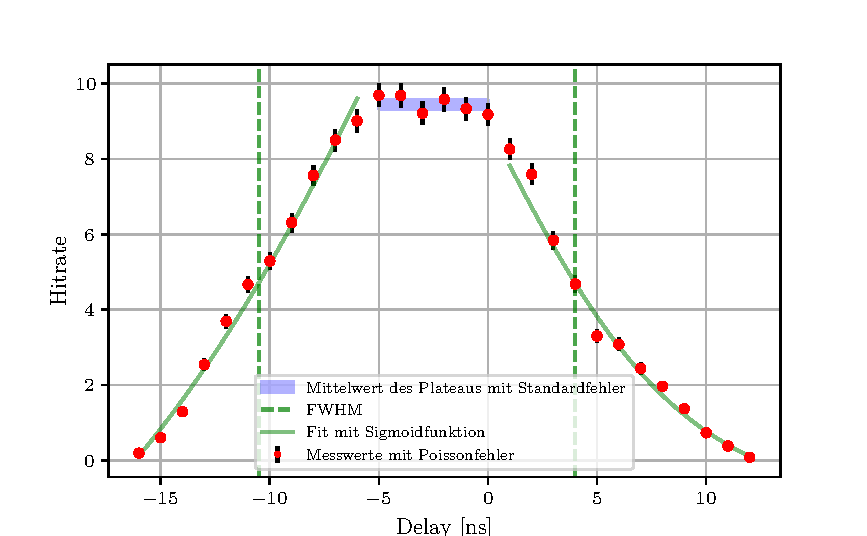
\includegraphics[width=0.95\textwidth]{build/delay.pdf}
  \caption{Hitrate in Abhängigkeit der Verzögerung.}
  \label{fig:kalibrierung}
\end{figure}

In \autoref{fig:kalibrierung} ist die Hitrate in Abhängigkeit der Verzögerung dargestellt. Es ist zu sehen, dass sich bei einer Verzögerung von -5 bis 0 ns ein Plateau in der Hitrate bildet. Da es sich innerhalb
des Plateaus um statistische Fluktuationen handelt, wird der Mittelwert als Maximum der Hitrate angenommen. Der Mittelwert der Hitrate innerhalb des Plateaus beträgt $\SI{9.44(0.13)}{s^{-1}}$.\\
Um nun über die Genauigkeit der Messapparatur Aussagen zu treffen, wird die Halbwertsbreite (auch FWHM) der Hitrate bestimmt. Die Halbwertsbreite ist der Bereich, in dem die Hitrate die Hälfte des Maximums beträgt.
Um die Halbwertsbreite zu bestimmen, wird links und rechts vom Plateau eine Sigmoidfunktion an die Messwerte angepasst. Die Sigmoidfunktion ist definiert als
\begin{equation*}
  f(x) = \frac{a}{1 + \exp(-b(x-c))} + d
\end{equation*}
wobei $a$, $b$, $c$ und $d$ die Parameter der Funktion sind. Die Parameter der Sigmoidfunktion werden mit der curve\_fit-Funktion von Scipy \cite{scipy} bestimmt und sind in \autoref{tab:sigmoid} aufgeführt.

\begin{table}[H]
  \centering
  \caption{Parameter der Sigmoidfunktionen.}
  \label{tab:sigmoid}
  \begin{tabular}{c|c|c}
    \hline
    \textbf{Parameter} & \textbf{Wert (links)} & \textbf{Wert (rechts)}\\
    \hline
    a & $\SI{11.64(1.57)}{}$ & $\SI{15.96(5.66)}{}$\\
    b & $\SI{0.39(0.07)}{}$ & $\SI{-0.27(0.08)}{}$\\
    c & $\SI{-10.90(0.42)}{}$ & $\SI{1.60(2.14)}{}$\\
    d & $\SI{-1.23(0.55)}{}$ & $\SI{-0.74(0.74)}{}$\\
    \hline
  \end{tabular}
\end{table}

Die Halbwertsbreite wird nun durch die Differenz der Schnittpunkte der Sigmoidfunktion mit der Hälfte des Maximums bestimmt und beträgt $\SI{14.79}{ns}$. Da an den Diskriminatorschwellen jeweils eine Pulsdauer
von $\SI{12(0.5)}{ns}$ eingestellt wurde, ergibt sich die Auflösungszeit zu
\begin{equation*}
  \Delta t = |2 \cdot \SI{12(0.5)}{ns} - \SI{14.79}{ns}| = \SI{9.2(1.0)}{ns}.
\end{equation*}

\subsection{Untergrundbereinigung}

Da es sich bei der Zählrate um eine Poisson-verteilte Größe handelt, kann damit auch der Untergrund abgeschätzt werden. 
Für die Zählrate gilt
\begin{equation*}
  Z = \frac{N_{start}}{T{ges}}.
\end{equation*}
Dabei ist $N_{start}$ die Anzahl der Startimpulse und $T_{ges}$ die gesamte Messzeit. Für die Poisson-Verteilung gilt dann 
\begin{equation*}
  P(k) = \frac{(Z \cdot t)^k}{k!} \cdot \exp(-Z \cdot t).
\end{equation*}
Die Wahrscheinlichkeit, dass ein weiterer Impuls nach einer Zeit $t$ auftritt, ist dann
\begin{equation*}
  P(1) = 
\end{equation*}

Die Untergrundzahl lässt sich also zu
\begin{equation*}
  N_{Untergrund} = N_{start} \cdot P(1)
\end{equation*}
abschätzen.

\subsection{Kalibrierung des Multichannelanalyzers}

Um die Channel des MCAs einer Zeit zuordnen zu können, wurden die Messwerte in \autoref{tab:mca} aufgenommen.

\begin{table}[H]
  \centering
  \caption{Messwerte zur Kalibrierung des Multichannelanalyzers.}
  \label{tab:mca}
  \begin{tabular}{c|c}
    \hline
    \textbf{Channel} & \textbf{Counts} \\
    \hline
    7 & 0.3\\
    30 & 0.8\\
    53 & 1.3\\
    76 & 1.8\\
    99 & 2.3\\
    122 & 2.8\\
    145 & 3.3\\
    168 & 3.8\\
    191 & 4.3\\
    214 & 4.8\\
    237 & 5.3\\
    260 & 5.8\\
    283 & 6.3\\
    306 & 6.8\\
    329 & 7.3\\
    352 & 7.8\\
    375 & 8.3\\
    398 & 8.8\\
    421 & 9.3\\
    445 & 9.8
  \end{tabular}
\end{table}

Die Messwerte aus \autoref{tab:mca} werden nun in \autoref{fig:mca} dargestellt. Die Messwerte werden an eine lineare Funktion der Form
\begin{equation*}
  f(x) = a \cdot x + b
\end{equation*}
angepasst. Die Parameter der linearen Funktion sind $a = \SI{0.021(0.00)}{}$ und $b = \SI{0.15(0.00)}{}$.

\begin{figure}[H]
  \centering
  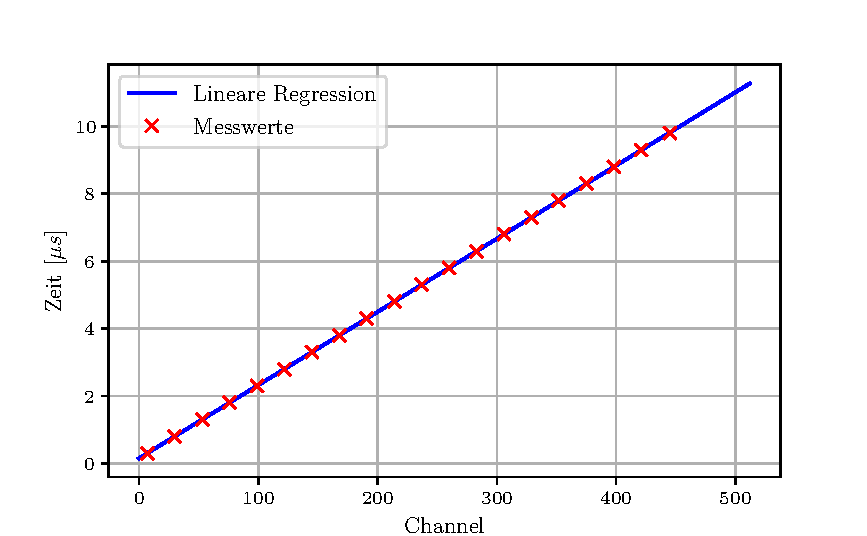
\includegraphics[width=0.95\textwidth]{build/mca.pdf}
  \caption{Messdaten und Ausgleichsgerade zur Kalibrierung des MCAs.}
  \label{fig:mca}
\end{figure}


%Plots und Bilder
%\begin{figure}[H]
%  \includegraphics[width=\linewidth]{plots/.pdf}
%  \caption{}
%  \label{fig:}
%\end{figure}

\newpage